\documentclass{article}
% pgfplots: Graphing library
\usepackage{pgfplots}

\begin{document}

\begin{figure}[h]
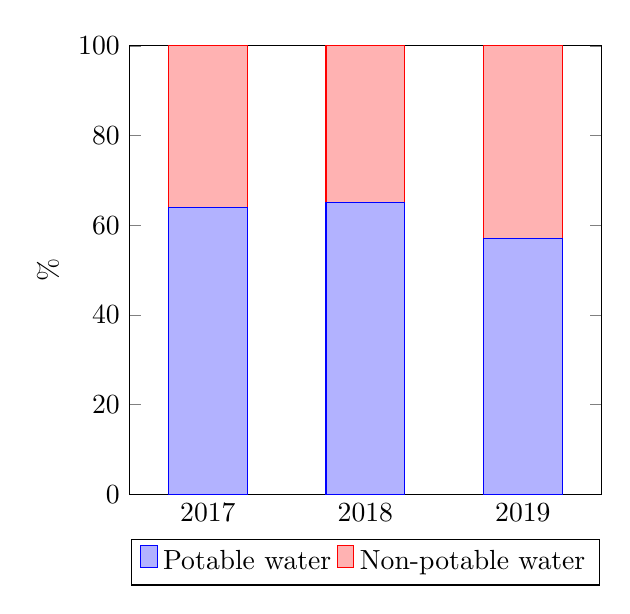
\begin{tikzpicture}
\begin{axis}[
    x tick label style={
		/pgf/number format/1000 sep=},
    xtick=data,
    ybar stacked,
    ylabel=\%,
    ymin=0,
    ymax=100,
    legend style={
        at={(0.5,-0.1)},
	    anchor=north,
        legend columns=-1
    },
    bar width=1cm,
    x=2cm,
    enlarge x limits={abs=1cm},
    enlarge y limits=false,
    ]
\addplot
coordinates {
    (2017,64) (2018,65) (2019,57)
};
\addplot
coordinates {
    (2017,36) (2018,35) (2019,43)
};
\legend{Potable water, Non-potable water}
\end{axis}
\end{tikzpicture}
\end{figure}

\end{document}
